\documentclass[aspectratio = 169]{beamer}
\usepackage[T1]{fontenc}

%%%%%%%% The beamer Theme %%%%%%%%%%%%%%%%%%%%%%
\usetheme{Rochester}
%\usetheme{metropolis}
%\usepackage[dvipdfmx]{graphicx}
\setbeamertemplate{navigation symbols}{}
%\usecolortheme{seagull}
%\usecolortheme{dove}
%\usecolortheme{owl}

%フラットデザインにする
\setbeamertemplate{blocks}[rounded] % Blockの影を消す
\useinnertheme{circles} % 箇条書きをシンプルに
\setbeamertemplate{navigation symbols}{} % ナビゲーションシンボルを消す
%\setbeamertemplate{headline}{}    %フレームタイトルの背景の色を消す
\setbeamertemplate{footline}[frame number] % フッターはスライド番号のみ
\renewcommand{\baselinestretch}{1.3}

%Beamerフォント設定
\usepackage[]{cmbright} %% Option 'defaultfam'
%% only if the base font of the document is to be sans serig
%\renewcommand*\oldstylenums[1]{{\fontfamily{Montserrat-TOsF}\selectfont #1}}

%\usepackage{newtxtext,newtxmath} % TXフォント
%\usepackage{sfmath}
%\usepackage[deluxe,uplatex]{otf} % 日本語多ウェイト化
%\renewcommand{\familydefault}{\sfdefault}  % 英文をサンセリフ体に
%\DeclareSymbolFont{operators}{OT1}{\sfdefault}{m}{n}
%\SetSymbolFont{operators}{bold}{OT1}{\sfdefault}{b}{n}
%\usepackage{mathrsfs}   %数式の文字をセリフに変える
%\usefonttheme{structurebold} % タイトル部を太字
%\setbeamerfont{alerted text}{series=\bfseries} % Alertを太字
%\setbeamerfont{section in toc}{series=\mdseries} % 目次は太字にしない
%\setbeamerfont{frametitle}{size=\Large} % フレームタイトル文字サイズ
%\setbeamerfont{title}{size=\LARGE} % タイトル文字サイズ
%\setbeamerfont{date}{size=\small}  % 日付文字サイズ

%%%%%%%%%%%%%% Packages %%%%%%%%%%%%%%%%%%%%%%
\usepackage{tikz}
\usepackage{bm}
\usepackage{natbib} % For reference https://gking.harvard.edu/files/natnotes2.pdf
\usepackage{multirow}
\usepackage{setspace}
\usepackage{booktabs}
\usepackage{float}
\usepackage{caption}
\usepackage{subcaption}

%%%%%%%%%%%%%%  Math Environment %%%%%%%%%%%%%% 
\usepackage{amsmath}
\usepackage{amsbsy}
\usepackage{ascmac}
\usepackage{amsthm}
\usepackage{amssymb}
\usepackage{mathtools}

%%%%%%% Theorem Environment based on amsthm %%%%%%%%%%%%%
\theoremstyle{definition}
\setbeamertemplate{theorems}[numbered] 
\newtheorem{thm}{Theorem}
\newtheorem{assm}{Assumption}
\newtheorem{lmma}{Lemma}
\newtheorem{prop}{Proposition}
\newtheorem{rslt}{Result}
\newtheorem{dfn}{Definition}
\newtheorem{crll}{Corollary}

\newtheorem{thm*}{Theorem}
\newtheorem{assm*}{Assumption}
\newtheorem{lmma*}{Lemma}
\newtheorem{prop*}{Proposition}
\newtheorem{rslt*}{Result}
\newtheorem{dfn*}{Definition}
\newtheorem{crll*}{Corollary}

\title{Revisiting Conduct Parameter Estimation in Homogeneous Goods Markets: At Least, Linear Model is Valid}
%\subtitle{Backus, Conlon, and Sinkinson, Working Paper, 2021}
\author{Yuri Matsumura and Suguru Otani}
\date{\today}

\begin{document}

\maketitle

\section{}
\begin{frame}{Introduction}
    \begin{itemize}
        \item Measuring competitiveness in markets is an important task in Empirical Industrial Organization
        \item We have some (in)direct measures of competitiveness and markup is the best-known measure
        \item As we cannot observe markup from data, one way to calculate markups is by fixing a model, estimating the model, and calculating the markup
        \item This way is suffered from misspecification
        \item Conduct parameter is another way that avoids misspecification because it uses a model that includes many competition models as special cases
    \end{itemize}
\end{frame}

\begin{frame}{Introduction}
    \begin{itemize}
        \item As for homogeneous product markets, the identification of the conduct parameter is guaranteed
        \begin{itemize}
            \item Bresnahan (1982) considers a linear demand and linear marginal cost model
            \item Lau(1982) considers a more general model
        \end{itemize}
        \item Perloff and Shen (2012) theoretically show that the linear model is suffered from the multicollinearity problem under some conditions
        \item They also conduct simulations to confirm their theoretical result
    \end{itemize}
\end{frame}


\begin{frame}{Results in PS(2012)}
    \begin{itemize}
        \item \textbf{Result 1}: The conduct parameter cannot be accurately estimated due to multicollinearity and nearly perfect collinearity problem
        \item \textbf{Result 2}: Using a log-linear demand and log-linear marginal cost model is recommended to avoid the multicollinearity problem
    \end{itemize}
\end{frame}

\begin{frame}{Our Result}
    \begin{itemize}
        \item \textbf{Result 1}: We can easily flip their conclusion by (1) properly adding demand shifters and (2) increasing the number of markets
        \begin{itemize}
            \item The simulation setting in PS (2012) has some problems
        \end{itemize}
        \item \textbf{Result 2}: Rather, the log-linear model cannot accurately estimate the conduct parameter due to the functional form of the supply equation
        \begin{itemize}
            \item The recommendation in PS (2012) is not helpful
        \end{itemize}
    \end{itemize}
\end{frame}


\begin{frame}{A Competition Model with Conduct Parameter}
    \begin{itemize}
        \item In homogeneous product markets, the supply equation is given as
        \begin{align*}
            P_t = -\theta\frac{\partial P_t}{\partial Q_t}Q_t + MC_t(Q_t),
        \end{align*}
        where $\theta$ is the conduct parameter
        \item When $\theta = 1$, the supply equation represents collusion, $\theta = 1/N$ represents Cournot, $\theta =0$ represents perfect competitive market
    \end{itemize}
\end{frame}




\begin{frame}{Identification of Conduct Parameter}
    \begin{itemize}
        \item Consider a linear demand and linear marginal cost model:
        \begin{align}
            P_t &= \alpha_0 - \alpha_1 Q_t + \alpha_2 Y_t + \varepsilon^{d}_{t},\label{eq:linear_demand}\\
            MC_t &= \gamma_0  + \gamma_1 Q + \gamma_2 W_{t} + \gamma_3 R_t + \varepsilon^{c}_{t},\label{eq:linear_marginal_cost}.
        \end{align}
        where $Y_t, W_t, R_t$ are exogenous variables and $\varepsilon^{d}_{t}$ and $\varepsilon^{c}_{t}$ are error terms
        \item The demand parameter $\alpha$ can be separately identified by the 2SLS
    \end{itemize}
\end{frame}

\begin{frame}{Identification of Conduct Parameter}
    \begin{itemize}
        \item In this case, the supply equation is written as
        \begin{align}
            P_t = \gamma_0 + (\theta\alpha_1 + \gamma_1) Q_t   + \gamma_2 W_{t} + \gamma_3 R_t + \varepsilon^{c}_{t}
        \end{align}
        \item We can identify $ \gamma_0, \gamma_2, \gamma_3$ and $\Gamma \equiv \theta\alpha_1 + \gamma_1$
        \item However, we cannot identify the conduct parameter $\theta = \frac{\Gamma - \gamma_1}{\alpha_1}$ because we don't know $\gamma_1$
    \end{itemize}
\end{frame}


\begin{frame}{Identification of Conduct Parameter}
    \begin{itemize}
        \item Bresnahan (1982) introduces a demand rotation IV $Z_t^R$:
        \begin{align}
            P_t &= \alpha_0 - (\alpha_1 + \alpha_2Z^{R}_{t})Q_t + \alpha_3 Y_t + \varepsilon^{d}_{t},\\
            MC_t &= \gamma_0  + \gamma_1 Q + \gamma_2 W_{t} + \gamma_3 R_t + \varepsilon^{c}_{t},.
        \end{align}
        \item In this case, the supply equation is written as
        \begin{align}
            P_t = \gamma_0 + [\theta(\alpha_1 + \alpha_2Z^{R}_{t})+ \gamma_1] Q_t   + \gamma_2 W_{t} + \gamma_3 R_t + \varepsilon^{c}_{t}
        \end{align}
    \end{itemize}
\end{frame}


\begin{frame}{Identification of Conduct Parameter}
    \begin{itemize}
        \item Further, we can have
        \begin{align}
            P_t = \gamma_0 + \theta(\alpha_1 +\alpha_2Z^{R}_{t})Q_t + \gamma_1 Q_t   + \gamma_2 W_{t} + \gamma_3 R_t + \varepsilon^{c}_{t}
        \end{align}
        \item As $(\alpha_1 +\alpha_2Z^{R}_{t})Q_t$ is an interaction term with the exogenous variable and the endogenous variable, we can identify $\theta$ and $\gamma_1$
    \end{itemize}
\end{frame}

\begin{frame}{Estimation of Conduct Parameter}
    \begin{itemize}
        \item Perloff and Shen (2012) show the linear model is suffered from the multicollinearity problem         
        when $\varepsilon^{d}_{t}$ and $\varepsilon^{c}_{t}$ are both zero
        \item When the standard deviation of the error terms is small, they claim that the nearly perfect collinearity problem occurs
        \item PS (2012) conduct simulations to confirm their theoretical result
    \end{itemize}
\end{frame}

\begin{frame}{Estimation results in Table 2 of from PS(2012)}
    \begin{table}[!htbp]
    \label{tb:linear_linear_sigma_Perloff_Shen}
    \begin{center}
        \begin{tabular}{cllll}
            \hline
            & $\sigma=0.001$ & $\sigma=0.5$ & $\sigma=1$ & $\sigma=2$ \\
            $\alpha_0$ & $10.00\ (0.001)$ & $9.96\ (0.33)$ & $9.86\ (0.65)$ & $9.46 (1.20)$ \\
            $\alpha_1$ & $1.00\ (0.004)$ & $0.99\ (1.98)$ & $0.97\ (3.96)$ & $0.88 (7.80)$ \\
            $\alpha_2$ & $1.00\ (0.004)$ & $0.99\ (0.21)$ & $0.97\ (0.42)$ & $0.87\ (0.82)$ \\
            $\gamma_1$ & $0.46\ (0.88)$ & $0.46\ (0.91)$ & $0.47\ (0.93)$ & $0.49\ (1.04)$ \\
            $\gamma_2$ & $5.85\ (7.89)$ & $5.85\ (8.15)$ & $5.78\ (8.21)$ & $5.73\ (8.66)$ \\
            $\theta$ & $-0.31\ (1.31)$ & $-0.29\ (1.34)$ & $0.09\ (11.48)$ & $-1.53\ (30.41)$ \\
            \hline
        \end{tabular}
    \end{center}
    \end{table}
    \begin{itemize}
        \item $\alpha_1 = \alpha_2 = \gamma_0 = \gamma_1 = \gamma_2  = \gamma_3 = 1, \alpha_0 = 10, \alpha_3 = 0,  \theta = 0.5, T = 50, R = 1000$
        \item $\varepsilon_t^d = \varepsilon_t^c \sim N(0,\sigma) $
    \end{itemize}
\end{frame}


\begin{frame}{Problems in PS(2012)}
    \begin{enumerate}
        \item Their simulation ignores demand shifter $Y_t$ by setting $\alpha_3 = 0$, that is, the supply estimation does not have any demand shifter
        \item It considers only one sample size in each simulation ($T = 50$) 
    \end{enumerate}
\end{frame}

\begin{frame}{Our simulation setting}
    \begin{itemize}
        \item We generate 1000 simulation data sets
        \item The parameter setting is the same as Perloff and Shen (2012), except we set $\alpha_3 = 1$
        \item We include demand shifter $Y_t$
        \item We apply the 2SLS for the demand and supply equation are done separately
        \item We also change the market size in each simulation ($T = 50, 100, 200, 1000$)
    \end{itemize}
\end{frame}

\begin{frame}{Result: Linear Model ($\sigma = 0.001$)}
    \begin{table}[]
        \centering
        \tiny
\begin{tabular}[t]{llrrrrrrr}
\toprule
  & Bias & RMSE & Bias & RMSE & Bias & RMSE & Bias & RMSE\\
\midrule
$\alpha_{0}$ & 0.000 & 0.001 & 0.000 & 0.001 & 0.000 & 0.000 & 0.000 & 0.000\\
$\alpha_{1}$ & 0.000 & 0.004 & 0.000 & 0.003 & 0.000 & 0.002 & 0.000 & 0.001\\
$\alpha_{2}$ & 0.000 & 0.000 & 0.000 & 0.000 & 0.000 & 0.000 & 0.000 & 0.000\\
$\alpha_{3}$ & 0.000 & 0.000 & 0.000 & 0.000 & 0.000 & 0.000 & 0.000 & 0.000\\
$\gamma_{0}$ & 0.000 & 0.001 & 0.000 & 0.001 & 0.000 & 0.001 & 0.000 & 0.000\\
$\gamma_{1}$ & 0.000 & 0.005 & 0.000 & 0.004 & 0.000 & 0.002 & 0.000 & 0.001\\
$\gamma_{2}$ & 0.000 & 0.000 & 0.000 & 0.000 & 0.000 & 0.000 & 0.000 & 0.000\\
$\gamma_{3}$ & 0.000 & 0.000 & 0.000 & 0.000 & 0.000 & 0.000 & 0.000 & 0.000\\
$\theta$ & 0.000 & 0.001 & 0.000 & 0.000 & 0.000 & 0.000 & 0.000 & 0.000\\
Sample size (n) &  & 50 &  & 100 &  & 200 &  & 1000\\
\bottomrule
\end{tabular}

        \label{tab:linear_with_demand_001}
    \end{table}
    \begin{itemize}
        \item Estimation with a demand shifter is almost perfect.
    \end{itemize}
\end{frame}

\begin{frame}{Result: Linear Model ($\sigma = 2$)}
    \begin{table}[]
        \centering
        \tiny
\begin{tabular}[t]{llrrrrrrr}
\toprule
  & Bias & RMSE & Bias & RMSE & Bias & RMSE & Bias & RMSE\\
\midrule
$\alpha_{0}$ & -0.263 & 2.596 & 0.071 & 1.670 & -0.040 & 0.947 & -0.002 & 0.412\\
$\alpha_{1}$ & -0.271 & 10.820 & 0.008 & 6.492 & 0.236 & 4.263 & 0.021 & 1.809\\
$\alpha_{2}$ & -0.044 & 1.253 & 0.023 & 0.779 & -0.031 & 0.483 & -0.003 & 0.210\\
$\alpha_{3}$ & -0.024 & 0.584 & 0.008 & 0.343 & -0.004 & 0.225 & 0.003 & 0.092\\
$\gamma_{0}$ & -2.074 & 19.624 & -0.551 & 3.043 & -0.171 & 1.516 & -0.051 & 0.633\\
$\gamma_{1}$ & 58.209 & 1750.688 & -2.416 & 56.909 & -3.617 & 39.044 & -0.103 & 2.334\\
$\gamma_{2}$ & 0.242 & 2.430 & 0.065 & 0.409 & 0.020 & 0.220 & 0.006 & 0.093\\
$\gamma_{3}$ & 0.230 & 2.328 & 0.055 & 0.404 & 0.010 & 0.219 & 0.008 & 0.092\\
$\theta$ & -6.668 & 233.851 & 0.372 & 6.334 & 0.418 & 3.820 & 0.024 & 0.245\\
Sample size ($T$) &  & 50 &  & 100 &  & 200 &  & 1000\\
\bottomrule
\end{tabular}

        \label{tab:linear_with_demand_2}
    \end{table}
    \begin{itemize}
        \item Sample size matters for estimation.
    \end{itemize}
\end{frame}



\begin{frame}{Log-linear model}
    \begin{itemize}
        \item Perloff and Shen (2012) claim that to avoid the multicollinearity and nearly perfect collinearity problem, the log-linear demand and log-linear model is a better specification
        \item Consider a log-linear demand and log-linear marginal cost;
        \begin{align}
            \log P_{t} &= \alpha_0 - (\alpha_1 + \alpha_2 Z^{R}_{t}) \log Q_t + \alpha_3 \log Y_t + \varepsilon^{d}_{t},\label{eq:log_linear_demand}\\
            \log MC_t &= \gamma_0 + \gamma_1 \log Q_t +  \gamma_2 \log W_{t} + \gamma_3 \log R_t + \varepsilon^{c}_{t}.\label{eq:log_linear_marginal_cost}
        \end{align}
    \end{itemize}
\end{frame}


\begin{frame}{Log-linear model}
    \begin{itemize}
        \item In this case, the supply equation is written as
        \begin{align}
            \log P_t = - \log(1 - \theta(\alpha_1 + \alpha_2 Z^{R}_{t})) + \gamma_0 + \gamma_1 \log Q_t +  \gamma_2 \log W_{t} + \gamma_3 \log R_t + \varepsilon^{c}_{t}
        \end{align}
        \item Lau (1982) guarantees the identification of the conduct parameter and the marginal cost parameters
    \end{itemize}
\end{frame}

\begin{frame}{Our simulation setting}
    \begin{itemize}
        \item We generate 1000 data sets under a slightly different parameter setting
        \item We still include the demand shifter
        \item The demand parameter is estimated by the 2SLS as it is a linear equation
        \item We apply the GMM for the supply estimation as it is a nonlinear equation
        \item We solve the minimization problem by using a nonlinear solver \texttt{IPOPT} with tolerance $10^{-6}$
    \end{itemize}
\end{frame}


\begin{frame}{Result: Log-linear Model ($\sigma = 0.001$)}
        \begin{table}[]
        \centering
        \tiny
\begin{tabular}[t]{llrrrrrrr}
\toprule
  & Bias & RMSE & Bias & RMSE & Bias & RMSE & Bias & RMSE\\
\midrule
$\alpha_{0}$ & 0.794 & 0.796 & 0.794 & 0.795 & 0.796 & 0.796 & 0.797 & 0.797\\
$\alpha_{1}$ & 0.000 & 0.114 & -0.002 & 0.075 & -0.002 & 0.045 & 0.000 & 0.018\\
$\alpha_{2}$ & 0.000 & 0.051 & 0.000 & 0.032 & -0.001 & 0.022 & 0.000 & 0.009\\
$\alpha_{3}$ & 0.859 & 0.868 & 0.857 & 0.861 & 0.854 & 0.856 & 0.857 & 0.857\\
$\gamma_{0}$ & -0.071 & 0.333 & -0.033 & 0.168 & -0.015 & 0.084 & -0.003 & 0.029\\
$\gamma_{1}$ & 0.000 & 0.001 & 0.000 & 0.000 & 0.000 & 0.000 & 0.000 & 0.000\\
$\gamma_{2}$ & 0.000 & 0.001 & 0.000 & 0.000 & 0.000 & 0.000 & 0.000 & 0.000\\
$\gamma_{3}$ & 0.000 & 0.000 & 0.000 & 0.000 & 0.000 & 0.000 & 0.000 & 0.000\\
$\theta$ & 0.014 & 0.382 & 0.016 & 0.081 & 0.009 & 0.052 & 0.002 & 0.020\\
Runs converged (\%) &  & 98.200 &  & 99.900 &  & 100.000 &  & 100.000\\
Sample size ($T$) &  & 50 &  & 100 &  & 200 &  & 1000\\
\bottomrule
\end{tabular}

        \label{tab:loglinear_with_demand_001}
    \end{table}
    \begin{itemize}
        \item Estimation with a demand shifter is almost perfect
    \end{itemize}
\end{frame}


\begin{frame}{Result: Log-linear Model ($\sigma = 2.0$)}
        \begin{table}[]
        \centering
        \tiny
\begin{tabular}[t]{llrrrrrrr}
\toprule
  & Bias & RMSE & Bias & RMSE & Bias & RMSE & Bias & RMSE\\
\midrule
$\alpha_{0}$ & -4.763 & 8.627 & -3.532 & 6.106 & -2.418 & 5.969 & -0.185 & 2.156\\
$\alpha_{1}$ & -1.066 & 1.853 & -0.786 & 1.353 & -0.540 & 1.339 & -0.043 & 0.480\\
$\alpha_{2}$ & -0.034 & 0.440 & -0.037 & 0.211 & -0.027 & 0.140 & 0.001 & 0.057\\
$\alpha_{3}$ & -0.519 & 0.936 & -0.389 & 0.709 & -0.255 & 0.637 & -0.018 & 0.247\\
$\gamma_{0}$ & -1.871 & 5.904 & -1.475 & 6.198 & -0.861 & 2.361 & -0.391 & 1.375\\
$\gamma_{1}$ & 0.281 & 1.305 & 0.201 & 1.526 & 0.058 & 0.399 & 0.013 & 0.147\\
$\gamma_{2}$ & 0.119 & 1.737 & 0.002 & 0.765 & 0.024 & 0.525 & 0.003 & 0.231\\
$\gamma_{3}$ & 0.123 & 0.690 & 0.090 & 1.111 & 0.026 & 0.260 & 0.005 & 0.101\\
$\theta$ & -2.205 & 10.866 & -0.636 & 36.600 & -1.289 & 9.693 & -0.463 & 4.420\\
Runs converged (\%) &  & 0.686 &  & 0.660 &  & 0.669 &  & 0.757\\
Sample size ($T$) &  & 50 &  & 100 &  & 200 &  & 1000\\
\bottomrule
\end{tabular}

        \label{tab:loglinear_with_demand_2}
    \end{table}
    \begin{itemize}
        \item When the sample size is $T = 1000$, the RMSE of the conduct parameter in the  linear model is 0.245, whereas the RMSE in the log-linear model is 4.42
        \item Run converged for 66-75\% of simulation samples
    \end{itemize}
\end{frame}

\begin{frame}{Summary of results: Log-linear Model}
    \begin{itemize}
        \item Increasing sample size and including demand shifter do not lead to accurate estimation results
        \begin{itemize}
            \item In particular, $\gamma_0$ and $\theta$
        \end{itemize}
        \item \textbf{Q: Why this happens?}
    \end{itemize}
\end{frame}

\begin{frame}{Histogram of the Simulation Result}
    \begin{figure}[!htbp]
      \begin{center}
          {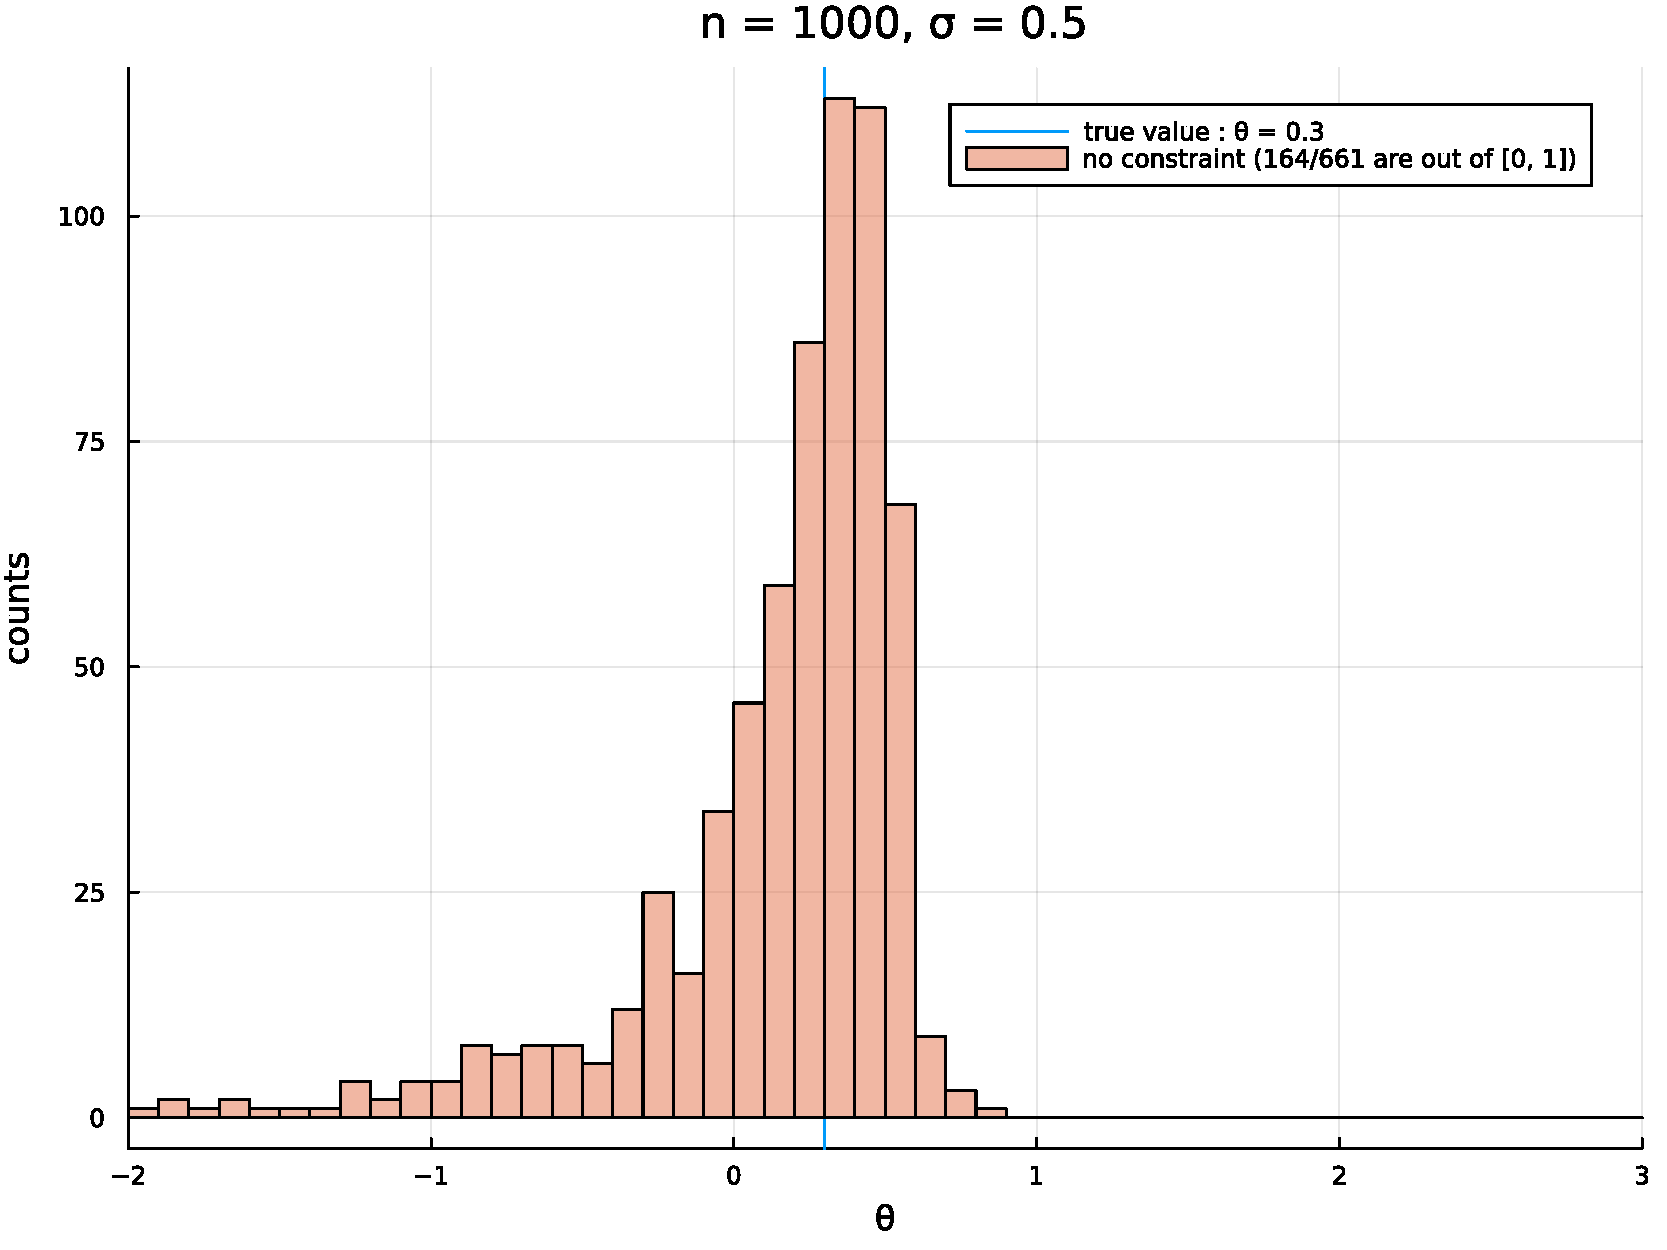
\includegraphics[width = 0.45\textwidth]
          {figuretable/histogram_loglinear_loglinear_n_1000_sigma_0.5_non_constraint.pdf}}
          {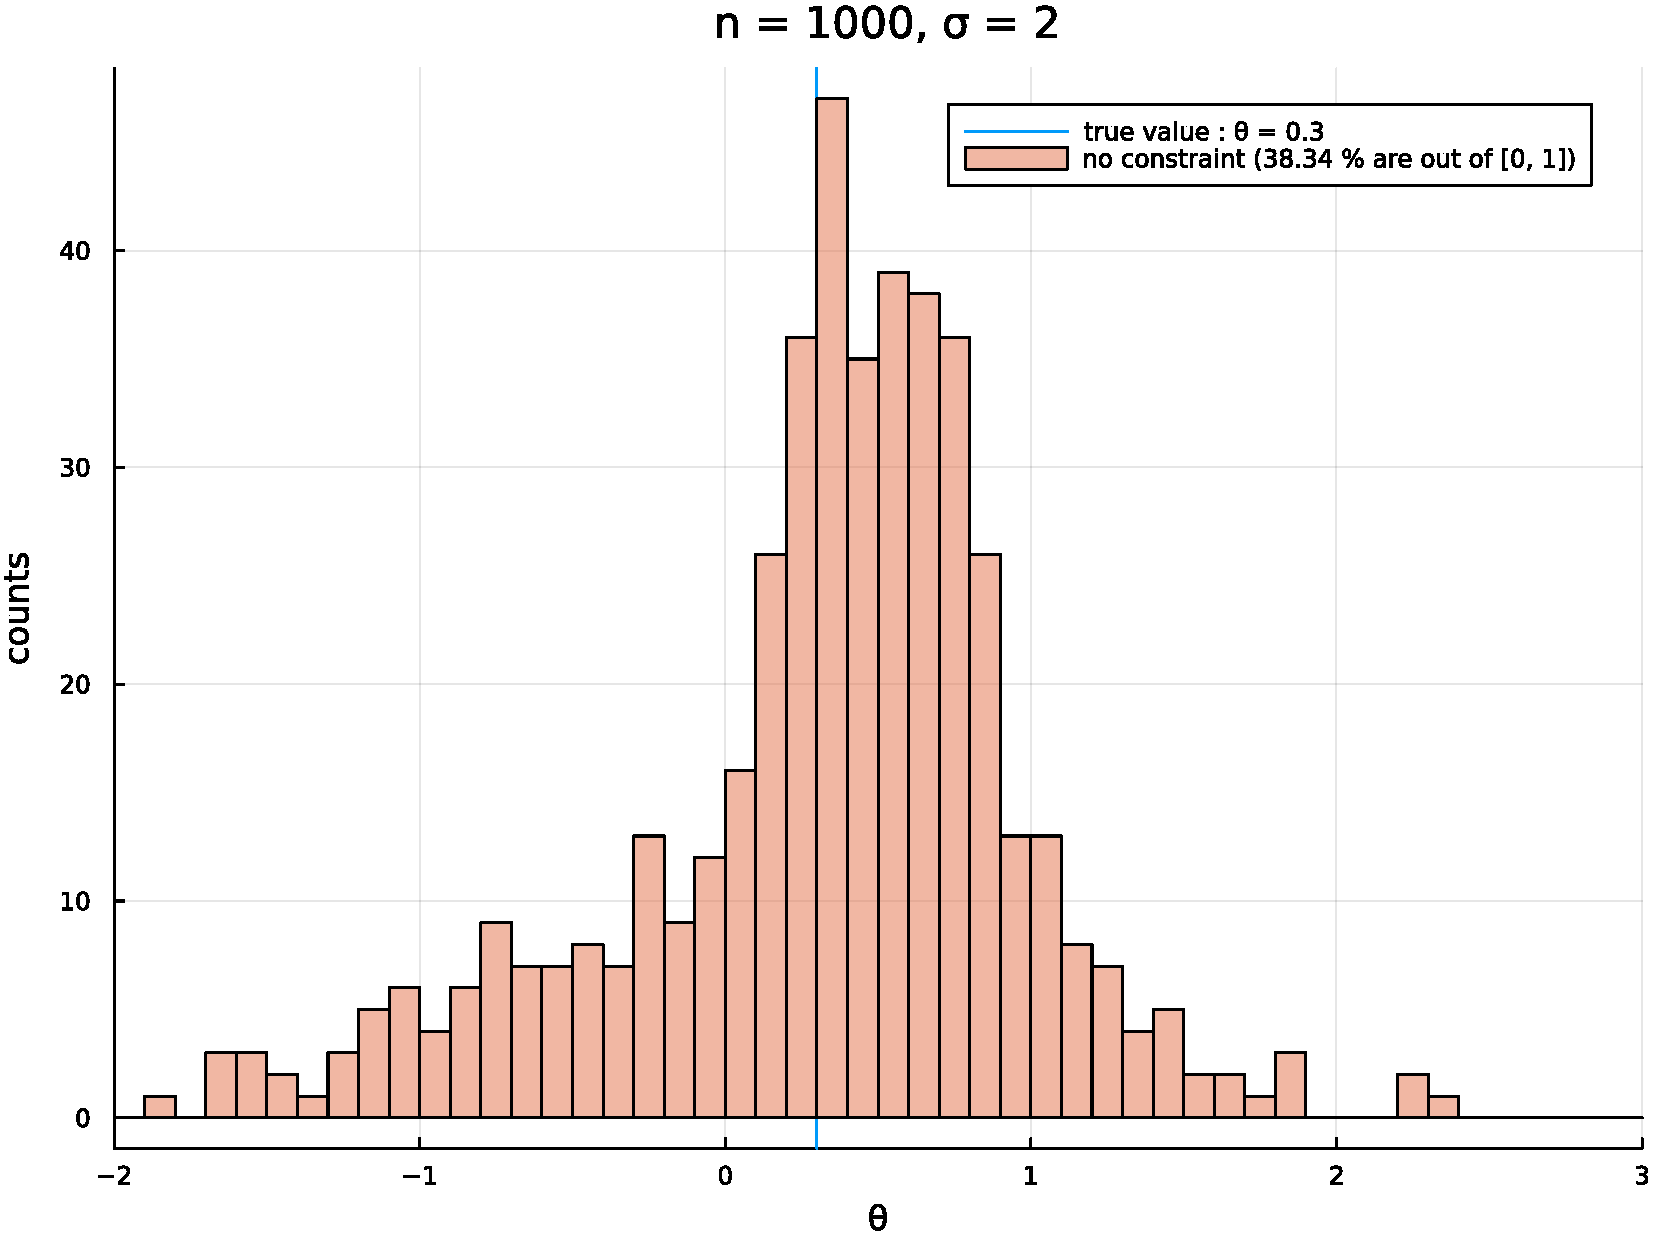
\includegraphics[width = 0.45\textwidth]
          {figuretable/histogram_loglinear_loglinear_n_1000_sigma_2_non_constraint.pdf}}
          \label{fg:histogram_loglinear_loglinear_no_constraint} 
        \end{center}
    \end{figure}
    \begin{itemize}
        \item The minimum values are $-329\ (\sigma = 0.5)$ and $-78\ (\sigma = 2)$
    \end{itemize}
\end{frame}



\begin{frame}{Intuitive Explanation}
    \begin{itemize}
        \item Recall that the conduct parameter is in the log function
            \begin{align*}
                \log P_t = \textcolor{purple}{- \log(1 - \theta(\alpha_1 + \alpha_2 Z^{R}_{t})) + \gamma_0} + \gamma_1 \log Q_t +  \gamma_2 \log W_{t} + \gamma_3 \log R_t + \varepsilon^{c}_{t}
            \end{align*}
        \item For example, when $\alpha_1 + \alpha_2 Z^{R}_{t} = 1$ and $\theta = - 78$, then $\log(79) = 1.8$
        \item When the value of $\theta$ is different from the true value, by adjusting the value of $\gamma_0$, we can decrease the value of the GMM
        \item There is a possibility that a nonlinear solver stops at unrealistic values of $\gamma_0$ and $\theta$
        \item To see whether this situation happens, we calculate the value of the GMM function under the true parameter and the estimated parameter
    \end{itemize}
\end{frame}

\begin{frame}{The Difference Between the GMM Values }
    \begin{figure}[!htbp]
  \begin{center}
  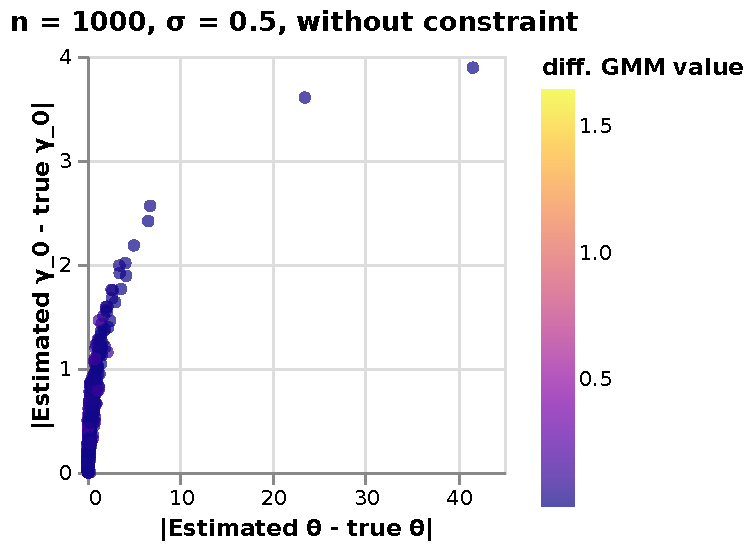
\includegraphics[width = 0.45\textwidth]
  {figuretable/diff_gmm_value_loglinear_loglinear_n_1000_sigma_0.5_non_constraint.pdf}
  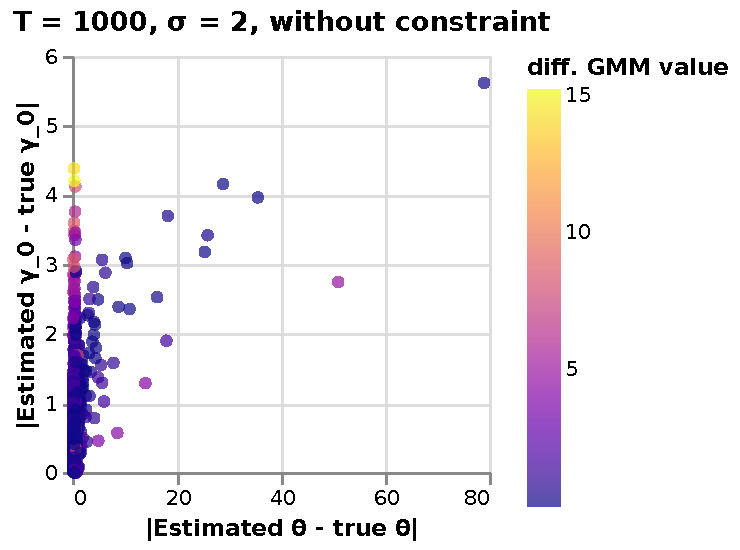
\includegraphics[width = 0.45\textwidth]
  {figuretable/diff_gmm_value_loglinear_loglinear_n_1000_sigma_2_non_constraint.pdf}
  \label{fg:diff_gmm_loglinear_loglinear} 
  \end{center}
\end{figure} 
\end{frame}



\begin{frame}{Summary}
    \begin{itemize}
        \item We reinvestigate the conduct parameter estimation in homogeneous product markets
        \item Unlike the conclusion in Perloff and Shen (2012), we find that the conduct parameter estimation in homogeneous product markets with the linear model can lead to accurate results
        \item While Perloff and Shen (2012) suggest using the log-linear model, we find the model is suffered from other estimation problems
    \end{itemize}
\end{frame}


\begin{frame}{}
    \centering
    \large Appendix
\end{frame}


\begin{frame}{The Contour Map of the GMM function}
    \begin{figure}
        \centering
        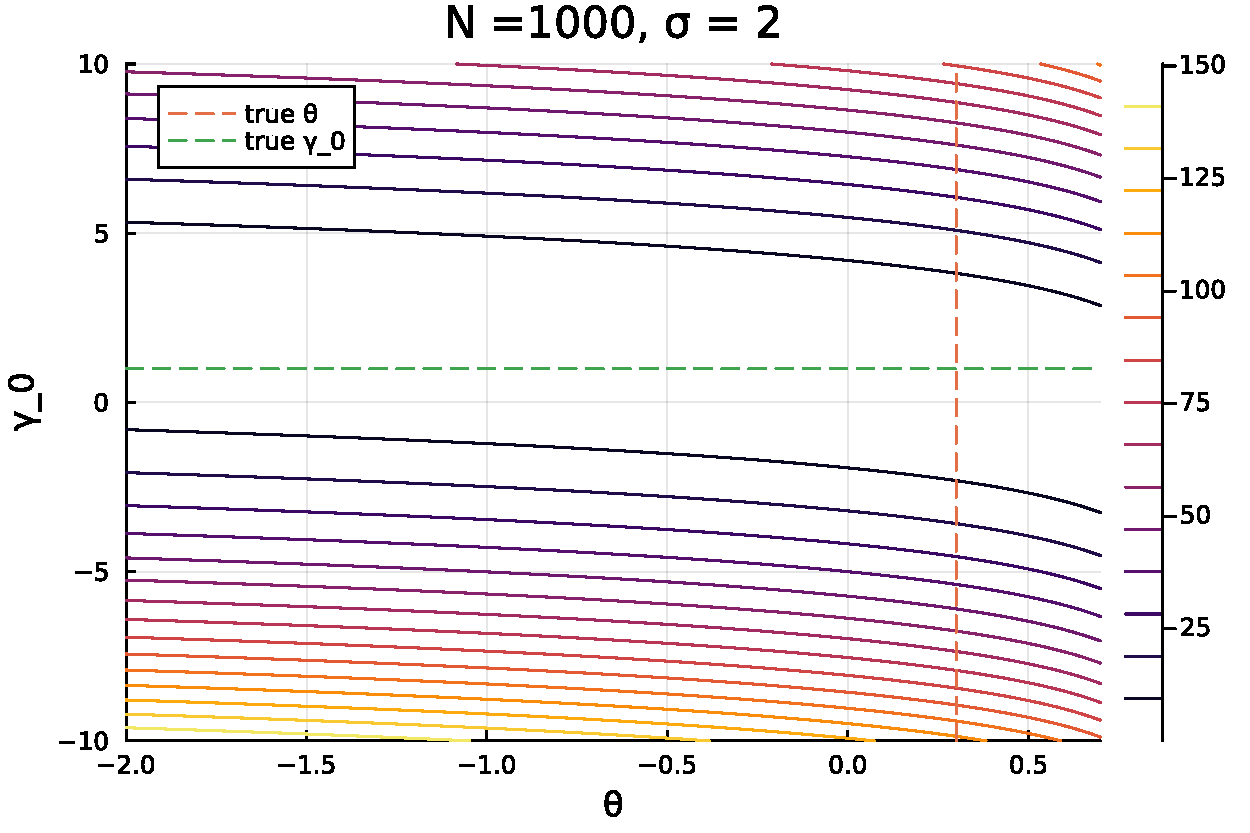
\includegraphics[width = 9cm]{figuretable/contour_loglinear_loglinear_n_1000_sigma_2.pdf}
        \label{fig:contour_map}
    \end{figure}
\end{frame}

\begin{frame}{Additional Results}
    \begin{itemize}
        \item We consider robustness for the choice of (1) a tolerance level and (2) starting value.
        \item We have used a tolerance $ = 10^{-6}$
        \item Can a tight tolerance solve the problem?
        \item We set the starting values to zero
        \item Can different starting values solve the problem?
    \end{itemize}
\end{frame}

\begin{frame}{Additional Results}
\begin{figure}
    \begin{subfigure}[b]{0.475\textwidth}
         \centering
         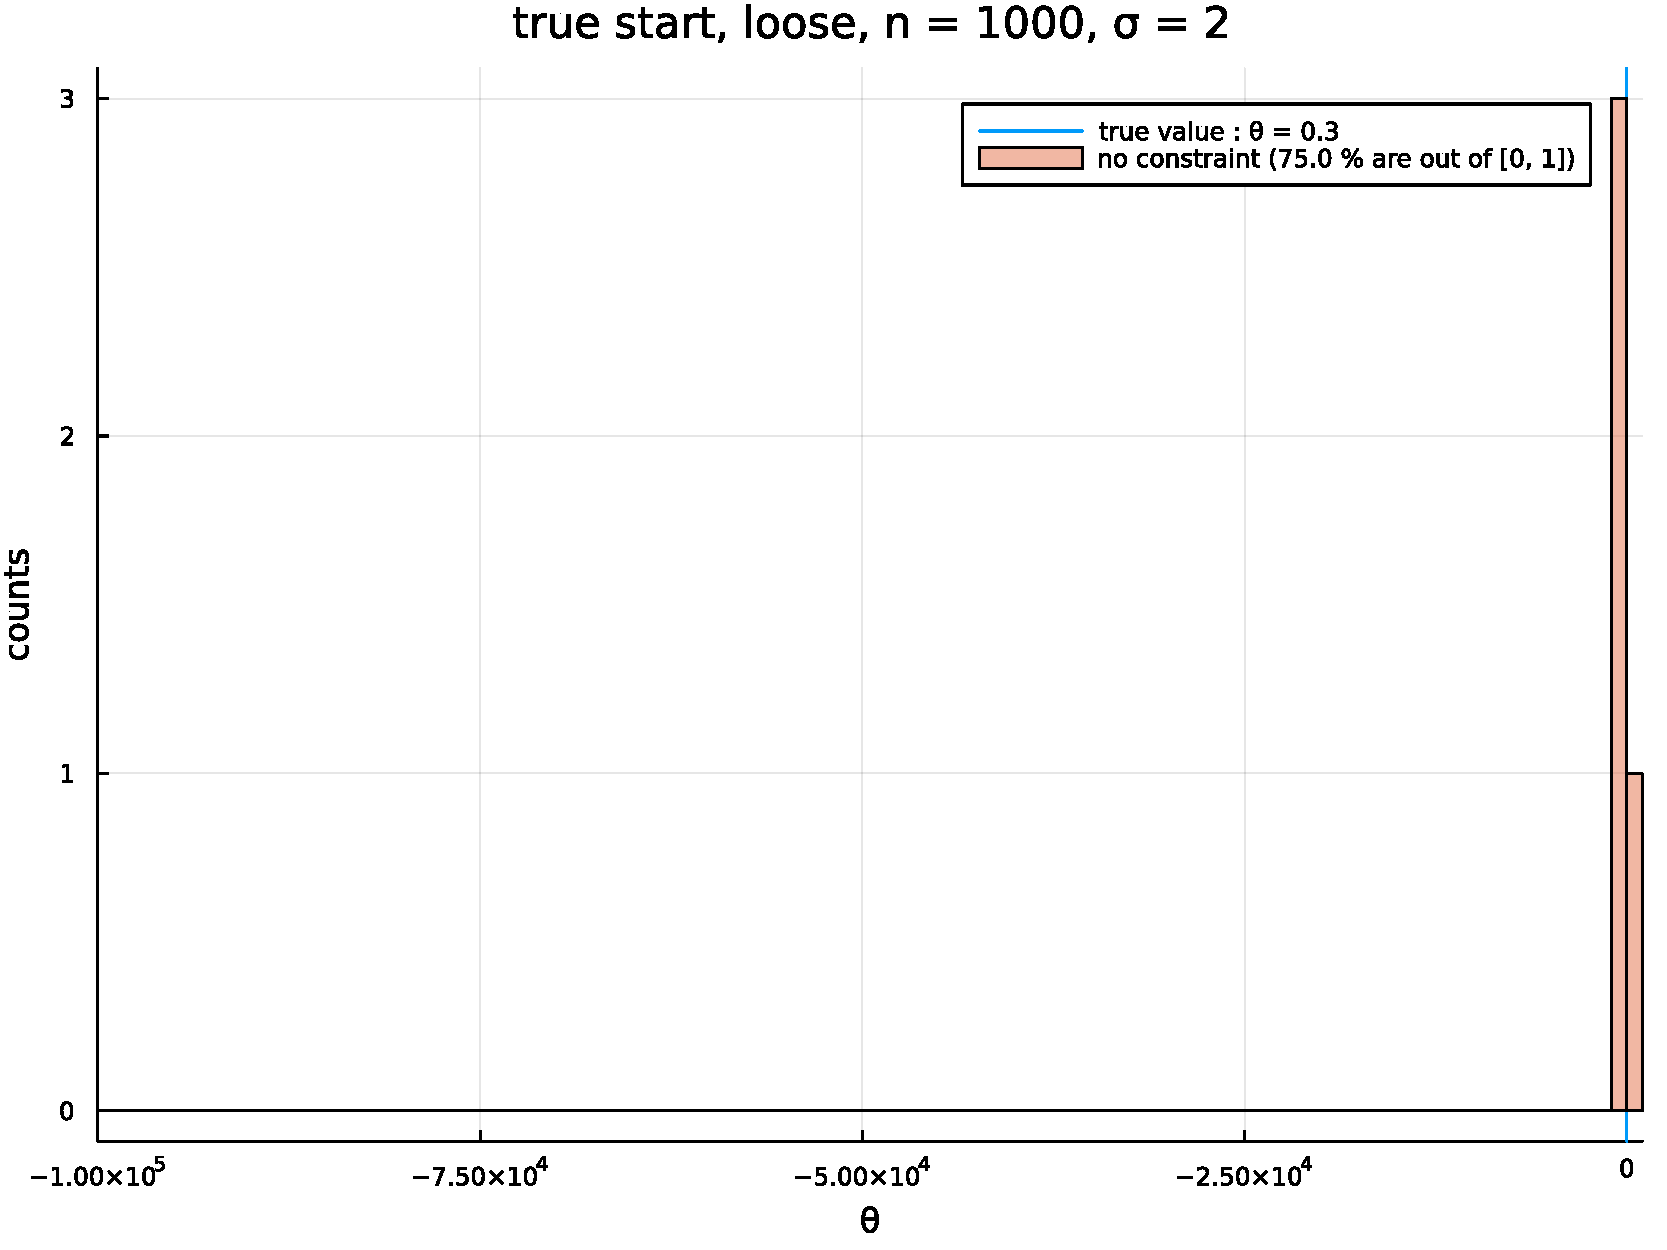
\includegraphics[width=\textwidth]{figuretable/loose/histogram_loglinear_loglinear_n_1000_sigma_2_non_constraint_true_start.pdf}
     \end{subfigure}
        \hfill
        \begin{subfigure}[b]{0.475\textwidth}
             \centering
             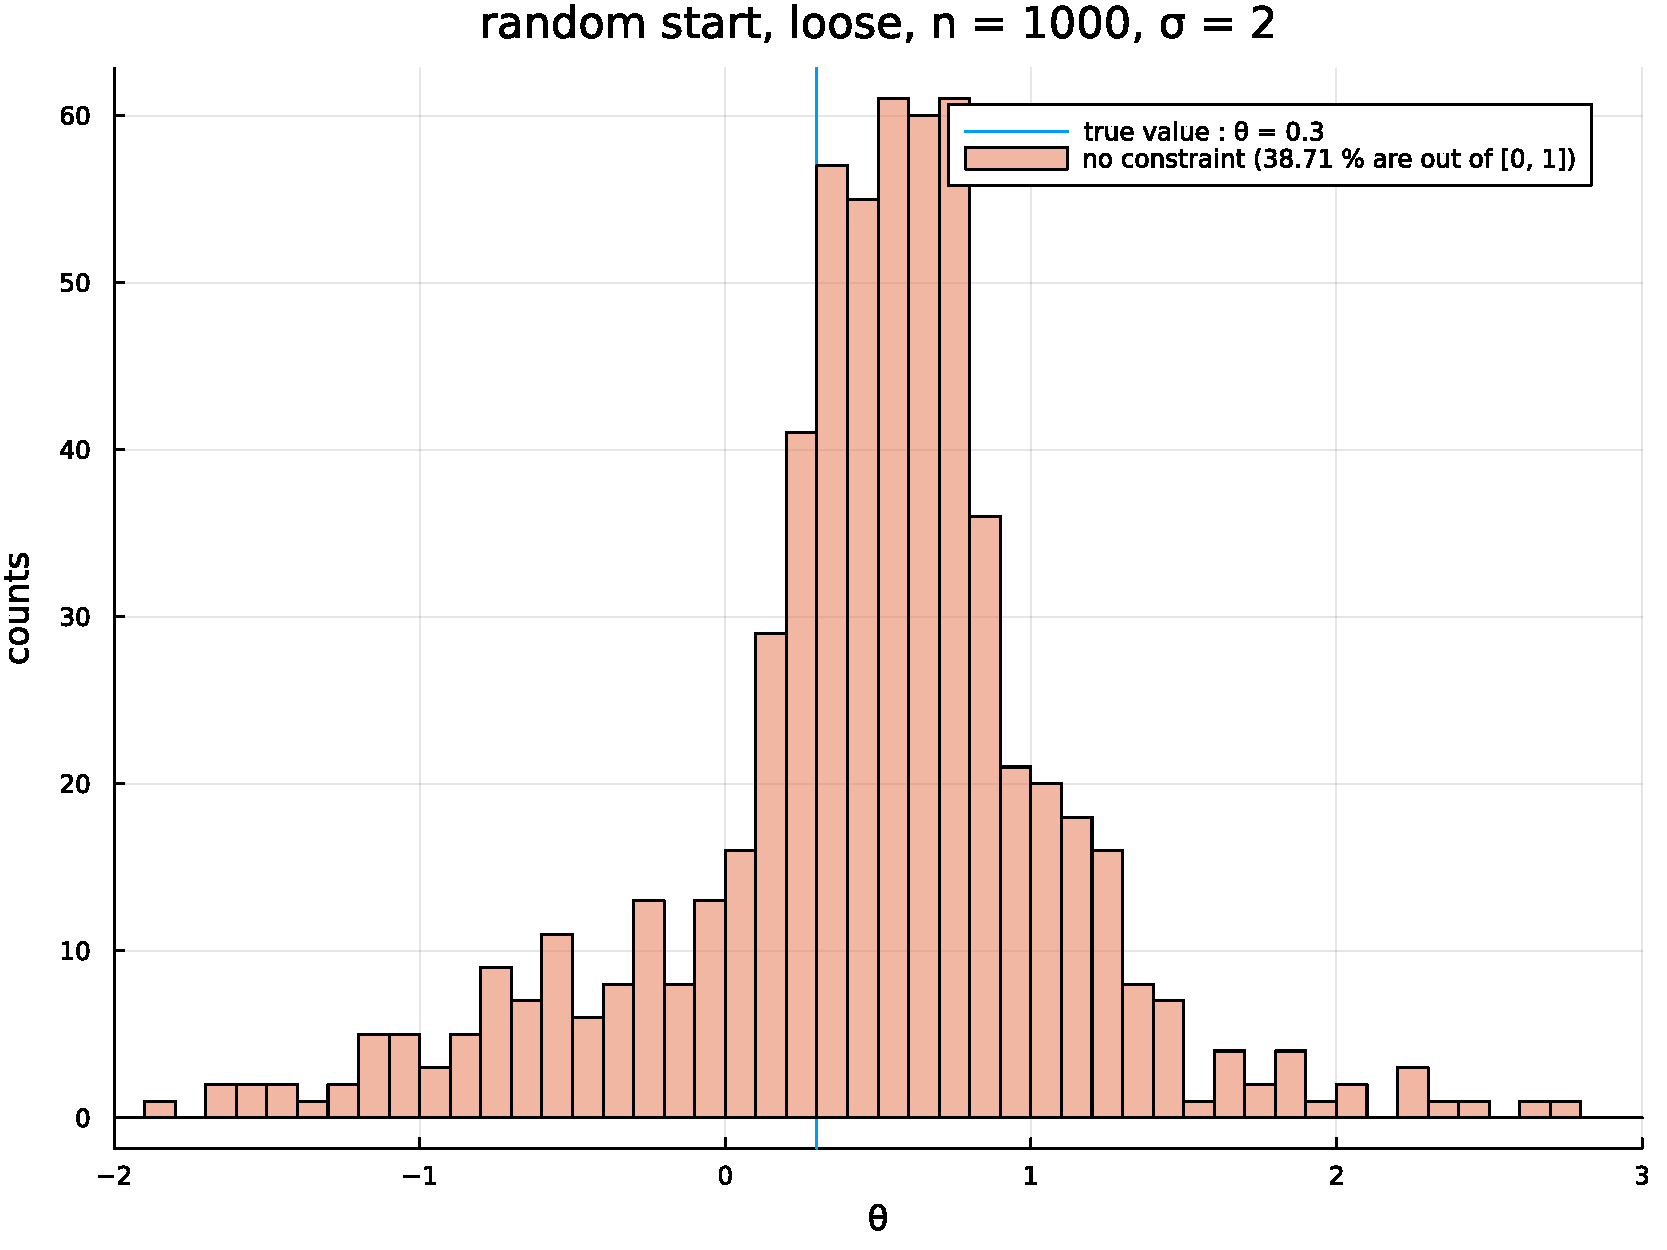
\includegraphics[width=\textwidth]{figuretable/loose/histogram_loglinear_loglinear_n_1000_sigma_2_non_constraint_random_start.pdf}
        \end{subfigure}
\end{figure}
\end{frame}


\begin{frame}{Additional Results}
\begin{figure}
    \begin{subfigure}[b]{0.475\textwidth}
         \centering
         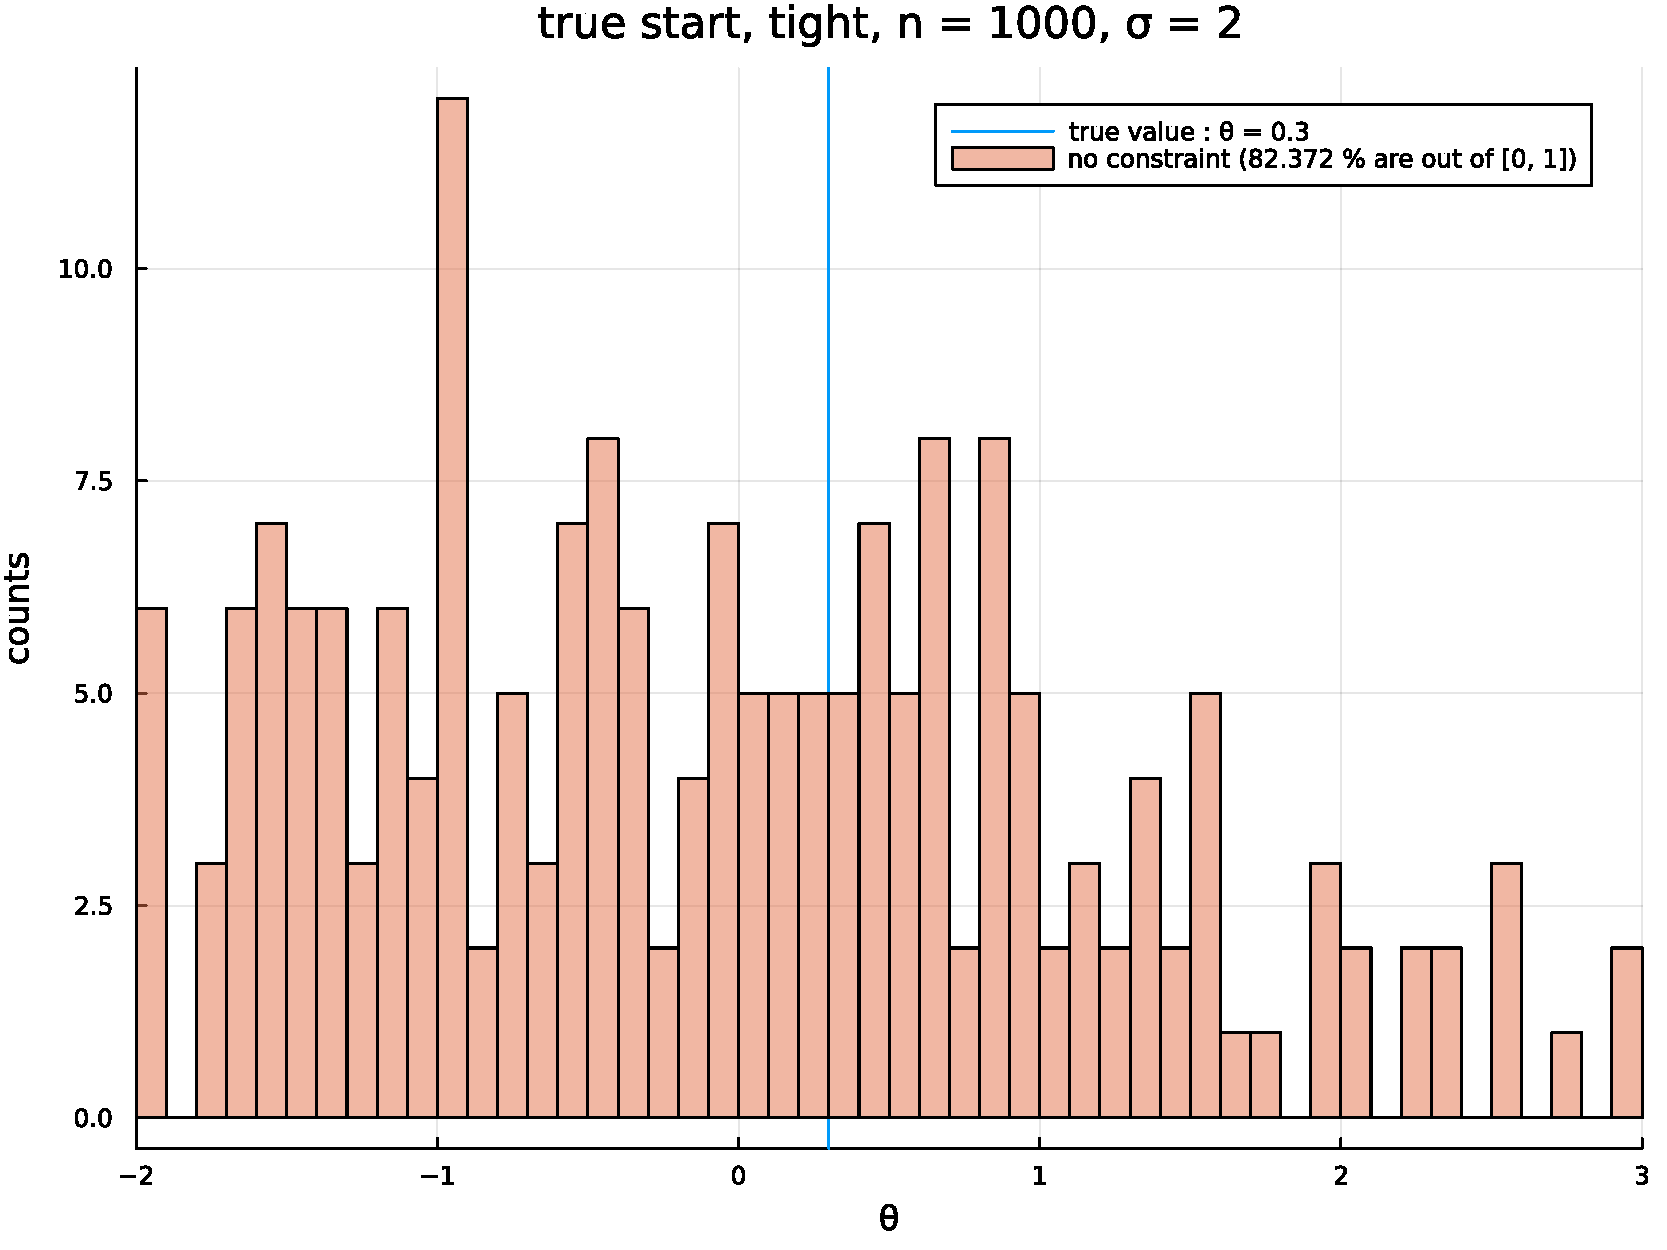
\includegraphics[width=\textwidth]{figuretable/tight/histogram_loglinear_loglinear_n_1000_sigma_2_non_constraint_true_start.pdf}
     \end{subfigure}
     \hfill
     \begin{subfigure}[b]{0.475\textwidth}
         \centering
         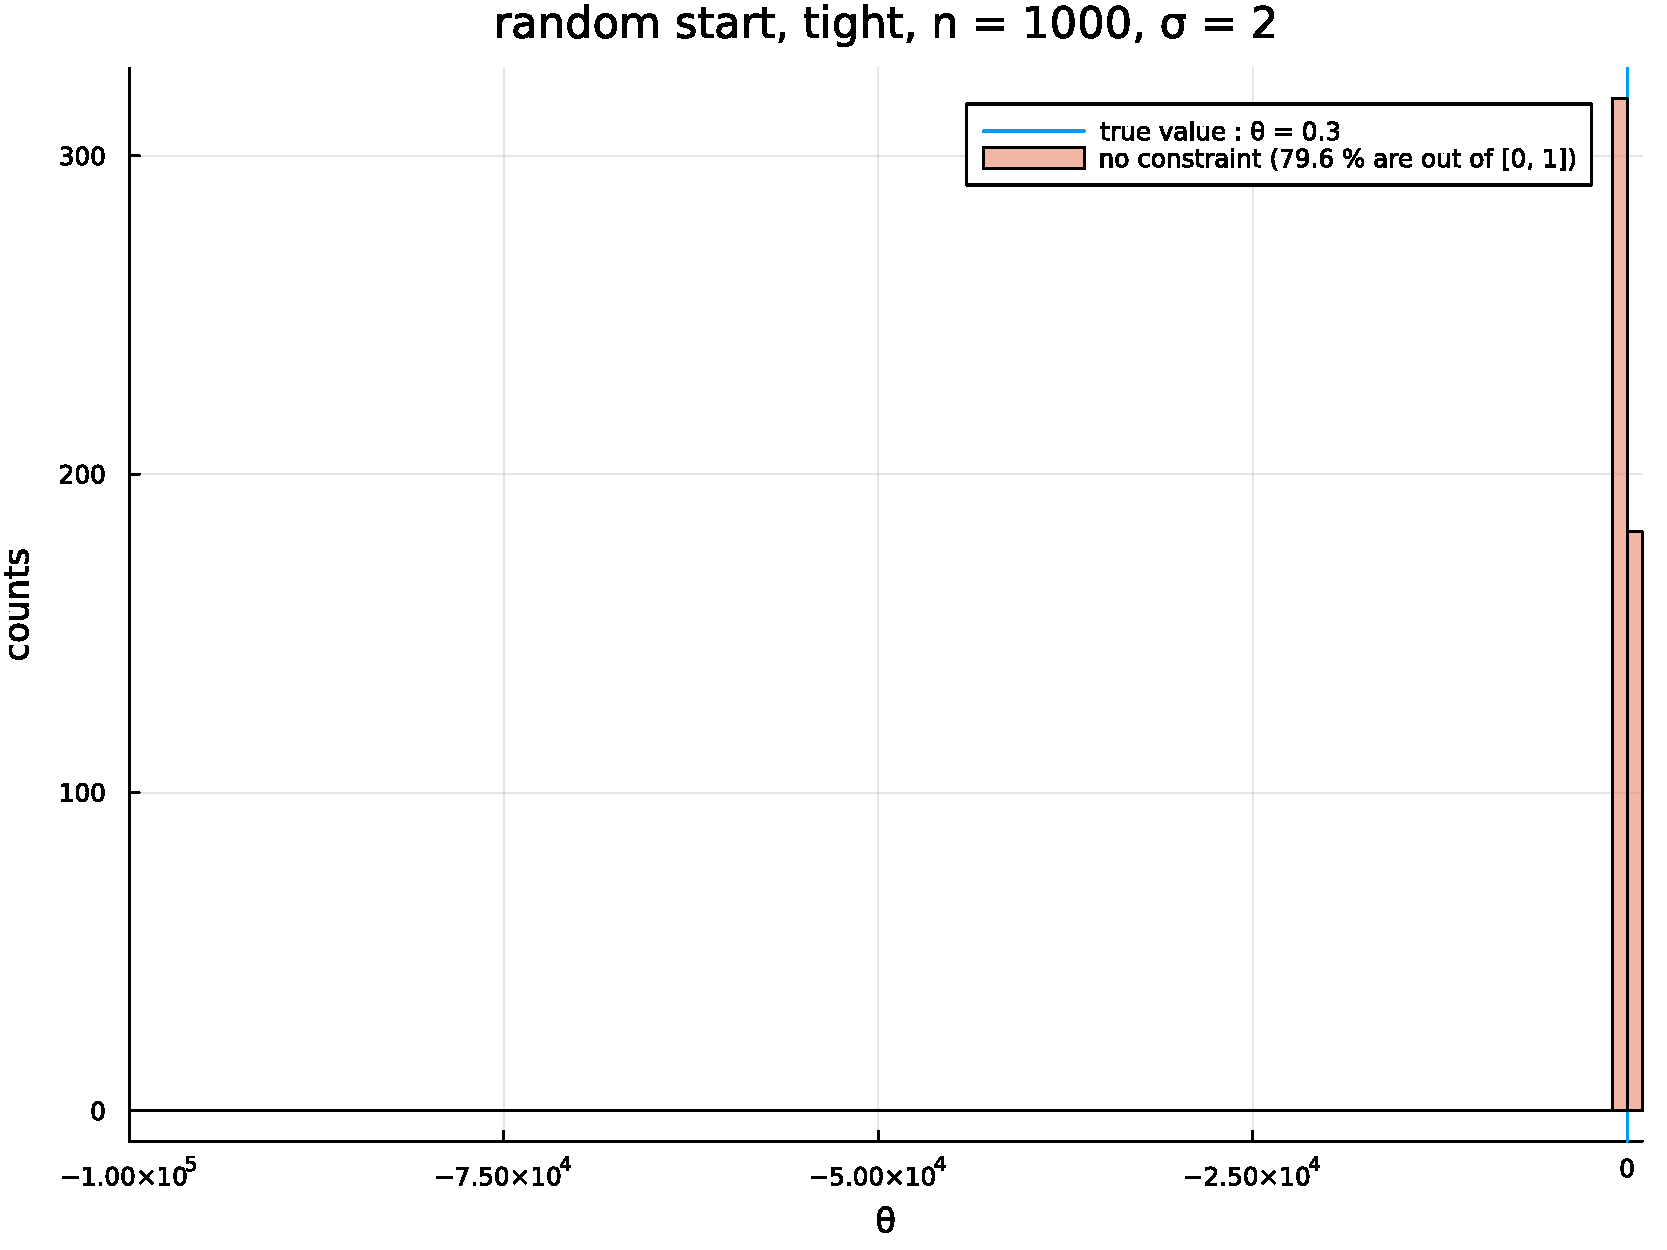
\includegraphics[width=\textwidth]{figuretable/tight/histogram_loglinear_loglinear_n_1000_sigma_2_non_constraint_random_start.pdf}
     \end{subfigure}
\end{figure}
\end{frame}


\end{document}